\documentclass[conference]{IEEEtran}
\IEEEoverridecommandlockouts
\usepackage{cite}
\usepackage{amsmath,amssymb,amsfonts}
\usepackage{graphicx}
\usepackage{textcomp}
\usepackage{xcolor}

\graphicspath{{../docs/figures/}}

\begin{document}

\title{Predictive Information in Conjunction Data-Message Histories Decays as Time to Closest Approach Decreases%
\thanks{Living manuscript (v2). Results are the 18 August 2026 freeze until later phases replace them. Unresolved items are marked as not yet measured.}}

\author{\IEEEauthorblockN{Arjun Vijay Prakash}
\IEEEauthorblockA{\textit{City Montessori School, Kanpur Road Campus}\\
Lucknow, India}
}

\maketitle

\begin{abstract}
Conjunction Data Messages (CDMs) report a collision probability that moves as later tracking shrinks orbital uncertainty. Operators often start planning about two days before closest approach, so an earlier forecast is useful only if the history available then contains information beyond copying the latest report. Using the public ESA Collision Avoidance Challenge archive, this study freezes the clock at 72, 48, 24, and 12 hours before closest approach and asks whether cutoff-safe summaries improve a forecast of the later reported log10 collision probability over persistence. On a leakage-safe hold-out of 1659 events, a gradient-boosted tree cuts mean absolute error from 5.080 to 2.808 at 48 hours, but persistence median absolute error is already 0: typical reports often do not move. The mean is dominated by rare jumps, including collapses to the dataset floor of -30. ESA-style loss (high-risk mean squared error divided by F2) ties at 0.167 once a persistence guard is applied on the log10 Pc at or above -6 class. The learned advantage is largest at 72 hours and nearly gone at 12 hours. Bootstrap 90 percent bands cover 47.7 percent of outcomes and are therefore model spread, not calibrated intervals. Later phases will add residual targets, a floor model, conformal coverage, and a one-shot score on official-test labels released in 2021. This is a research prototype, not flight software.
\end{abstract}

\begin{IEEEkeywords}
conjunction data message, collision probability, space debris, forecast horizon, gradient boosting, persistence
\end{IEEEkeywords}

\section{Introduction}

Two orbiting objects can pass close enough to generate a conjunction alert. The reported collision probability $P_c$ is not a physical constant: it is recomputed as radar and optical observations shrink (or fail to shrink) the combined covariance~\cite{ccsdsCdm,hejduk2016}. Waiting usually improves the estimate and leaves less time to plan. ESA posed the forecasting form of this problem in the 2019 Collision Avoidance Challenge: predict the final reported $\log_{10} P_c$ from messages with time to closest approach of at least two days~\cite{uriot2021,esaKelvins}. Persistence---copying the latest pre-cutoff risk---was a strong baseline. Only 12 of 96 teams beat it on ESA-style loss.

That competition does not answer how the extra information, if any, depends on remaining time, nor whether a mean-error win is a typical-event win. Physics-based $P_c$ forecasting via expected covariance reduction~\cite{duncan2014} and operational work on probability dilution~\cite{alfano2003,hejduk2016} suggest that large early covariances can make $P_c$ look safely small, then later updates either collapse risk to negligible or concentrate it. A recent machine-learning model predicts which conjunctions will keep high covariance, for extra tracking~\cite{stauch2026}. The target here is different: the later reported $\log_{10} P_c$ itself, under a frozen information cutoff.

The working hypotheses are as follows.
\begin{itemize}
\item H1: Extra predictive information beyond copying the latest report is largest at long horizons and approaches zero near closest approach.
\item H2: Most of the mean-error win is rare floor jumps, not typical events becoming more accurate.
\item H3: Extra information does not automatically improve high-risk decisions under the ESA class $\log_{10} P_c \ge -6$.
\item H4 (\textit{not yet measured}): The snapshot gap between \texttt{max\_risk\_estimate} and \texttt{risk}, together with large covariance, predicts later $|\Delta\mathrm{risk}|$ and floor collapse.
\end{itemize}

\section{Methods}

\subsection{Data}
Labeled CDMs from the ESA training archive comprise 162{,}634 rows and 13{,}154 events, 2015--2019, anonymized~\cite{esaKelvins}. Events need a message at or before the cutoff and a later labeled update. That yields 8{,}293 eligible events at 48 hours before closest approach. Train, validation, calibration, and test are event-disjoint (3{,}731 / 1{,}659 / 1{,}244 / 1{,}659). Features use only rows with time to closest approach at or above the cutoff. The later $\log_{10} P_c$ is the label, never an input.

\subsection{Model}
The current selected policy is event-level XGBoost on inspectable snapshot and history summaries, with a ten-model bootstrap median and a persistence guard when the current report is already at or above $-6$. Baselines are persistence, the training-set median, and Ridge. Official Kelvins test inputs are schema-checked only in this freeze; labeled official-test scoring is \textit{not yet measured} (planned one-shot evaluation using labels released on Zenodo in 2021~\cite{esaKelvins}).

\subsection{Metrics}
Reported scores are mean and median absolute error in $\log_{10} P_c$, the share within 0.5 log units, and ESA-style loss $L=\mathrm{MSE}_{HR}/F_2$ with $\beta=2$ on the $-6$ class~\cite{uriot2021}. Floor-excluded MAE, residual MAE, bootstrap confidence intervals, conformal coverage, and official-test $L$ are \textit{not yet measured}.

The 18 August freeze was re-run through plot generation, lint, unit tests, and a production website build without retraining, so Tables~\ref{tab:scoreboard} and~\ref{tab:horizon} are unchanged. The product specification and exhibit UI were left alone until a later phase selects a replacement policy on validation.

\section{Results}

Table~\ref{tab:scoreboard} reports the frozen local test. Column ``0.5'' is the share of events within 0.5 log units; ``HR'' is high-risk MAE. Persistence median absolute error is 0: more than half of later reports do not move by a measurable amount after 48 hours. The selected policy ties persistence on ESA-style loss because the guard copies any current report already in the scored tail. Unguarded XGBoost has better MAE and $F_2=0$. The constant median beats the selected policy on MAE. These facts are the content of H2 and H3 on this freeze; they are not a scoring bug.

\begin{table}[t]
\caption{Local test at 48 hours ($n=1659$). MAE in $\log_{10} P_c$. Selected policy: bootstrap ensemble with a $-6$ persistence guard.}
\label{tab:scoreboard}
\begin{center}
\scriptsize
\begin{tabular}{|l|r|r|r|r|r|}
\hline
\textbf{System} & \textbf{MAE} & \textbf{Med.} & \textbf{0.5} & \textbf{HR} & $\boldsymbol{L}$/$\boldsymbol{F_2}$ \\
\hline
Persistence & 5.080 & 0.000 & 63.1\% & 0.89 & 0.167/0.361 \\
\hline
Train.\ median & 3.002 & 0.000 & 81.6\% & 24.8 & ---/0 \\
\hline
Unguarded XGB & 2.808 & 0.557 & 48.8\% & 13.69 & ---/0 \\
\hline
Selected ens. & 3.059 & 0.474 & 50.5\% & 3.69 & 0.167/0.361 \\
\hline
\end{tabular}
\end{center}
\end{table}

Table~\ref{tab:horizon} and Fig.~\ref{fig:horizon} support H1 on this freeze: the learned advantage shrinks as closest approach approaches. The 12-hour gap is 0.06 log units and is \textit{not yet} equipped with a confidence interval.

\begin{table}[t]
\caption{Single XGBoost versus persistence by horizon. MAE in $\log_{10} P_c$. The 72~h and 12~h eligible sets overlap the 48~h split but are not identical.}
\label{tab:horizon}
\begin{center}
\begin{tabular}{|l|r|r|r|}
\hline
\textbf{Horizon} & \textbf{XGBoost} & \textbf{Persist.} & \textbf{Adv.} \\
\hline
72 h & 3.214 & 7.748 & 4.534 \\
\hline
48 h & 2.808 & 5.080 & 2.272 \\
\hline
24 h & 2.110 & 2.634 & 0.524 \\
\hline
12 h & 1.384 & 1.444 & 0.060 \\
\hline
\end{tabular}
\end{center}
\end{table}

\begin{figure}[t]
\centerline{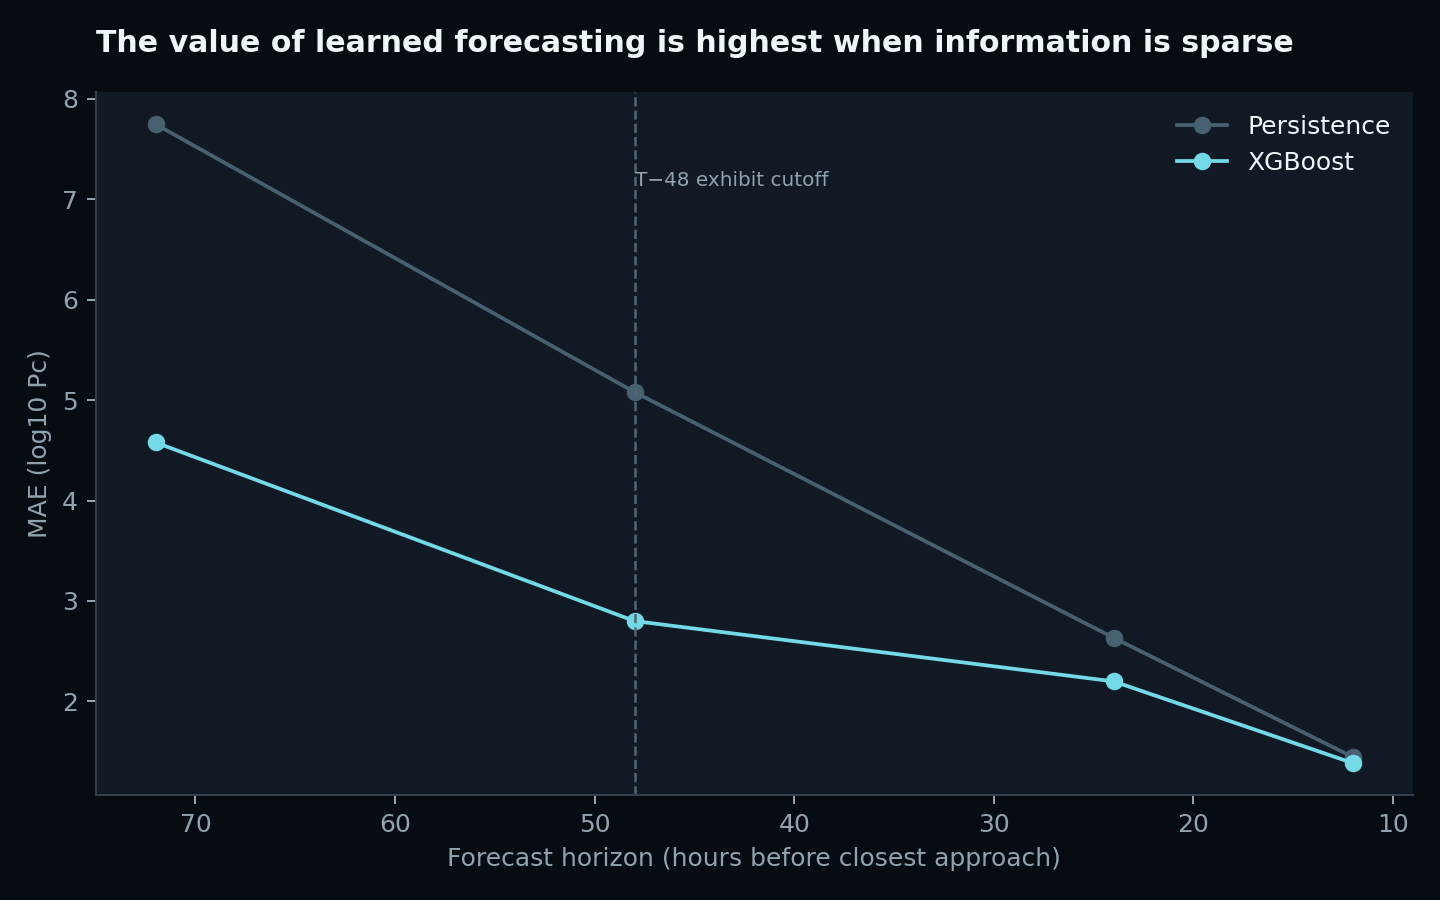
\includegraphics[width=\columnwidth]{forecast-horizon.png}}
\caption{Forecast-horizon MAE for the learned model and persistence (18 August freeze).}
\label{fig:horizon}
\end{figure}

Snapshot-only MAE is 2.904; adding historical summaries of the same fields lowers it to 2.851; covariance trends reach 2.808. History therefore adds a small increment that also still needs an interval.

Nominal 50\% and 90\% bootstrap bands cover 25.8\% and 47.7\% of outcomes. They are reported as model spread. Conformal intervals are \textit{not yet measured}. One accepted high-risk miss remains (false reassurance $=1$ of 9 local high-risk test events). A four-mission hold-out has high-risk MAE 19.2 on a single held-out high-risk event.

\section{Discussion}

The 2019 challenge already showed that beating persistence on ESA-style loss is hard~\cite{uriot2021}. The contribution attempted here is not a second leaderboard entry. It is a measurement of \emph{when} CDM history still contains extra information, and of the fact that mean error and high-risk decisions are different jobs. Large early covariance can dilute $P_c$~\cite{alfano2003}; later contraction often drops reported risk~\cite{hejduk2016}. That physical picture matches a horizon-dependent learned advantage and a mean wrecked by floor collapses. It does not match a claim of operational warning skill on nine local positives.

This freeze uses historical ESA-supported missions from 2015 to 2019, not live catalogues. The local test has nine events at $\log_{10} P_c \ge -6$. Manoeuvres are out of scope. SHAP explains the fitted model, not physical causation. Official-test labels exist~\cite{esaKelvins} and have not yet been scored in this freeze.

Next measurements are floor-aware metrics and confidence intervals; a residual-to-persistence target; a two-part floor model; split-conformal coverage; a frozen official-test evaluation; a dilution-gap probe for H4; and repeated grouped splits.

\section*{Acknowledgment}

This work uses the ESA Space Debris Office Collision Avoidance Challenge dataset~\cite{esaKelvins,uriot2021}. ESA, ISRO, NASA, ISTRAC, and CCSDS did not endorse this project.

\bibliographystyle{IEEEtran}
\bibliography{references}

\end{document}
